\documentclass[tikz,border=2pt]{standalone}
\usepackage{pgfplots}
\usetikzlibrary{intersections}
\usepgfplotslibrary{fillbetween}
\pgfplotsset{compat=1.7}

\begin{document}
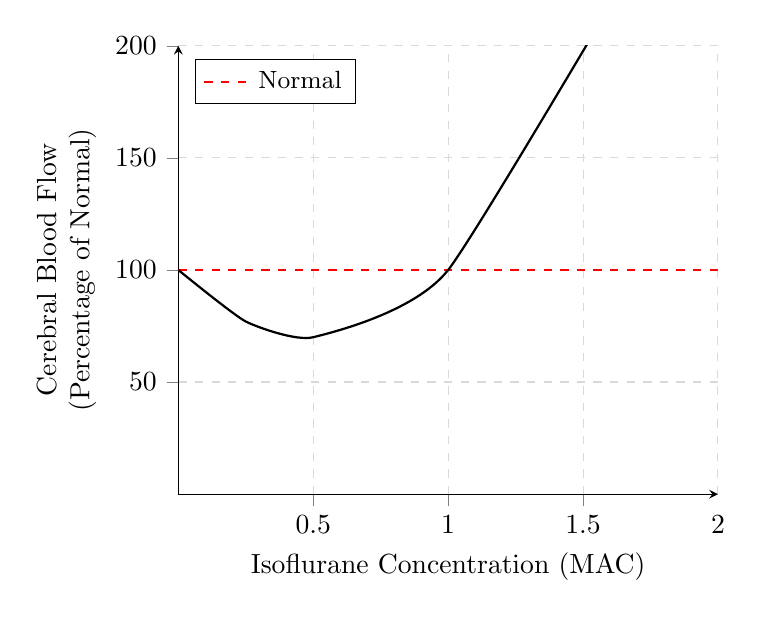
\begin{tikzpicture}


\begin{axis}[
        axis lines=middle,
        grid = major,
        grid style={dashed, gray!30},
	ymin = 0,
	ymax = 200,
	xmin = 0,
	xmax =2,
	 ylabel near ticks,
	xlabel near ticks,
        xlabel=Isoflurane Concentration (MAC),
        ylabel=Cerebral Blood Flow \\ (Percentage of Normal),
        tick align=outside,
        enlargelimits=false,
ylabel style={align=center},
legend pos= north west,
legend style={font=\small, cells={align=left}}]

\addplot[red,dashed,thick, domain=0:2] {100};
\addlegendentry{Normal};
\draw[black, thick] plot[smooth,tension=0.3] coordinates { (axis cs: 0,100) (axis cs: 0.25, 77) (axis cs: 0.5,70) (axis cs: 1,100) (axis cs: 2, 300)};

\end{axis}

\end{tikzpicture} 
\end{document}